\documentclass{article}

\usepackage{arxiv}

\usepackage[utf8]{inputenc} % allow utf-8 input
\usepackage[T1]{fontenc}    % use 8-bit T1 fonts
\usepackage{lmodern}        % https://github.com/rstudio/rticles/issues/343
\usepackage{hyperref}       % hyperlinks
\usepackage{url}            % simple URL typesetting
\usepackage{booktabs}       % professional-quality tables
\usepackage{amsfonts}       % blackboard math symbols
\usepackage{nicefrac}       % compact symbols for 1/2, etc.
\usepackage{microtype}      % microtypography
\usepackage{graphicx}

\title{Missing links, forbidden links, and the topological robustness of
food webs}

\author{
    Anubhav Gupta
    \thanks{Corresponding author}
   \\
    Department of Evolutionary Biology and Environmental Studies \\
    University of Zurich \\
  8057 Zurich, Switzerland \\
  \texttt{\href{mailto:anubhav.gupta@ieu.uzh.ch}{\nolinkurl{anubhav.gupta@ieu.uzh.ch}}} \\
   \And
    Owen L. Petchey
   \\
    Department of Evolutionary Biology and Environmental Studies \\
    University of Zurich \\
  8057 Zurich, Switzerland \\
  \texttt{\href{mailto:owen.petchey@ieu.uzh.ch}{\nolinkurl{owen.petchey@ieu.uzh.ch}}} \\
  }


% tightlist command for lists without linebreak
\providecommand{\tightlist}{%
  \setlength{\itemsep}{0pt}\setlength{\parskip}{0pt}}


% Pandoc citation processing
\newlength{\cslhangindent}
\setlength{\cslhangindent}{1.5em}
\newlength{\csllabelwidth}
\setlength{\csllabelwidth}{3em}
\newlength{\cslentryspacingunit} % times entry-spacing
\setlength{\cslentryspacingunit}{\parskip}
% for Pandoc 2.8 to 2.10.1
\newenvironment{cslreferences}%
  {}%
  {\par}
% For Pandoc 2.11+
\newenvironment{CSLReferences}[2] % #1 hanging-ident, #2 entry spacing
 {% don't indent paragraphs
  \setlength{\parindent}{0pt}
  % turn on hanging indent if param 1 is 1
  \ifodd #1
  \let\oldpar\par
  \def\par{\hangindent=\cslhangindent\oldpar}
  \fi
  % set entry spacing
  \setlength{\parskip}{#2\cslentryspacingunit}
 }%
 {}
\usepackage{calc}
\newcommand{\CSLBlock}[1]{#1\hfill\break}
\newcommand{\CSLLeftMargin}[1]{\parbox[t]{\csllabelwidth}{#1}}
\newcommand{\CSLRightInline}[1]{\parbox[t]{\linewidth - \csllabelwidth}{#1}\break}
\newcommand{\CSLIndent}[1]{\hspace{\cslhangindent}#1}

\usepackage{lineno}
\linenumbers
\usepackage {amsmath}
\setlength\parindent{24pt}
\usepackage{setspace}\doublespacing
\usepackage{booktabs}
\usepackage{longtable}
\usepackage{array}
\usepackage{multirow}
\usepackage{wrapfig}
\usepackage{float}
\usepackage{colortbl}
\usepackage{pdflscape}
\usepackage{tabu}
\usepackage{threeparttable}
\usepackage{threeparttablex}
\usepackage[normalem]{ulem}
\usepackage{makecell}
\usepackage{xcolor}
\begin{document}
\maketitle


\begin{abstract}
\begin{enumerate}
\def\labelenumi{\arabic{enumi})}
\tightlist
\item
  Undersampling can lead to missing trophic interactions in recorded
  food webs, with potential consequences for the perceived functioning
  and stability of the food web. Undersampling can be compensated for by
  using food web models such as allometric diet breadth model (ADBM) to
  predict missing links. Simultaneously, models might predict links
  which cannot occur, i.e., false positives.
\item
  Previous research shows that (i) food web robustness (the inverse of
  the number of secondary extinctions occuring due to primary
  extinctions) increases with connectance (the number of trophic links
  divided by the number of possible links), and (ii) that predicted food
  webs usually have greater connectance than observed ones. Thus we
  expect that predicted food webs are more robust than observed ones.
  This expectation has never, to our knowledge, been tested, nor has the
  effect size been quantified.
\item
  We fill this research gap by comparing the robustness of observed food
  webs to the robustness of food webs predicted by a model (the ADBM)
  that can account for missing links, though can also make false
  positives. We did this for 12 different food webs from a wide variety
  of ecosystems.
\item
  We found, as expected, that the predicted food webs were more robust
  than the observed food webs, and this can be attributed to the higher
  connectance of the predicted food webs. On average, for every X unit
  of increase in connectance, we found the food webs to be robust by YY
  units for random extinction scenario.\textbf{OP: Here something about
  the effect size.}
\item
  These results show that undersampling can lead to large underestimates
  of food web robustness that can be compensated for by filling in
  missing links with food web models. Nevertheless, increased
  connectance may contribute to lower dynamical stability, and so it
  would be interesting to compare the dynamical stability of observed
  and predicted food webs, as well as the topological stability that we
  have focused on.
\end{enumerate}
\end{abstract}

\keywords{
    connectance
   \and
    ABC
   \and
    ADBM
   \and
    food web
   \and
    extinction
   \and
    uncertainty
  }

\hypertarget{introduction}{%
\section{Introduction}\label{introduction}}

\hypertarget{background-on-anthropogenic-changes-and-its-impact-on-food-web}{%
\subsection{Background on anthropogenic changes and its impact on food
web}\label{background-on-anthropogenic-changes-and-its-impact-on-food-web}}

Anthropogenic changes such as climate change and habitat destruction are
a threat to biodiversity, and can lead to food web collapse (Ullah et
al. 2018). This collapse in the food web is due to cascades of secondary
extinctions in a food web because of primary loss of species, for
example due to habitat destruction. The rate of collapse of these
predicted food webs is dependent on the structure and complexity of
those food webs (Jennifer A. Dunne, Williams, and Martinez 2002b;
Jennifer A. Dunne and Williams 2009). Therefore, research focused on
cascading secondary extinctions also known as `community viability
analysis' have been performed extensively in the past few decades
(Jennifer A. Dunne, Williams, and Martinez 2002b; Jennifer A. Dunne and
Williams 2009; Berg et al. 2011; Ebenman, Law, and Borrvall 2004;
Ebenman and Jonsson 2005).

\hypertarget{briefly-explain-work-done-by-jennifer-dunne-on-food-web-op-robustness-to-primary-extinctions-and-also-what-has-been-done-since-particularly-concerning-the-importance-of-connectance}{%
\subsection{Briefly explain work done by Jennifer Dunne on food web
{[}OP{]} robustness to primary extinctions, and also what has been done
since, particularly concerning the importance of
connectance}\label{briefly-explain-work-done-by-jennifer-dunne-on-food-web-op-robustness-to-primary-extinctions-and-also-what-has-been-done-since-particularly-concerning-the-importance-of-connectance}}

Simulation of primary species loss has been conducted in observed food
webs and model food webs from terrestrial and aquatic ecosystems where
robustness was measured in terms of secondary extinctions (Jennifer A.
Dunne, Williams, and Martinez 2002b; Jennifer A. Dunne and Williams
2009). These studies showed that the robustness \textbf{of the food
webs} increases with food web connectance. Also, the removal of the most
connected species cause considerably more secondary extinctions than
random removals of species (Jennifer A. Dunne, Williams, and Martinez
2002a; Sol'e and Montoya 2001). These studies provide an alternate
solution to investigate the impact of primary extinctions in a food web
when canonical experiments in natural ecosystems are not possible.

Along with robustness based on topological structure of a food web,
robustness based on the food web dynamics has been studied as well
(reference). Topological approaches only require the food web structure
whereas dynamical approaches also require the temporal dynamics of the
food web along with the food web structure. For example: Williams (2008)
combined models of network structure with models of bionergetic dynamics
to study the role of food web topology and nonlinear dynamics on species
coexistence in complex ecological networks.

{[}OP{]} Explain (either here or in the methods) difference between
topological and abundance (given by dynamics) based criteria for a
secondary extinction occurring.

\hypertarget{op-state-what-is-the-problem}{%
\subsection{{[}OP{]} State what is the
problem\ldots{}}\label{op-state-what-is-the-problem}}

A key assumption of the observed food webs is that the food webs are
very well sampled i.e.~all the links that in reality can occur are
represented. However, it is known that not all food webs are very well
sampled and then do not represent all of the feeding links that occur
(Caron et al. 2022; Patonai and Jord'an 2017; Jordano 2016). Some rare
trophic links require more sampling effort as compared to others whereas
some trophic links remain unobserved because of linkage constraints
irrespective of sufficient sampling effort (Jordano 2016). One solution
to this problem is to use a food web model such as Allometric Diet
Breadth Model (ADBM) to predict which are the missing links, and to then
measure the robustness of the predicted food web. ADBM is a mechanistic
model constructed using rules based on body sizes of prey and predator
where trophic interactions satisfying those rules would be predicted by
the model which at the same time are perhaps not observed because those
interactions are rare. However, this solution is not infallible, as it
is likely that the food web model might still miss some links, and also
may predict some links that could not, in fact occur.

\hypertarget{what-we-do-in-this-study}{%
\subsection{What we do in this study}\label{what-we-do-in-this-study}}

In our study, we investigate the robustness of the ADBM predicted food
webs as compared to the observed food webs and quantify the effect of
overestimation of connectance on the robustness of these predicted food
webs. We do this by simulating primary species loss in 12 food webs
predicted from the ADBM to quantify the secondary loss of extinctions.
We use three different approaches of species removal: (i) most connected
species, (ii) random species and (iii) least connected species to
understand if the outcome varies among these approaches.

It is crucial to investigate the implication of this consistent
overestimation of connectance in the robustness of predicted food webs.
We expect that the ADBM predicted food webs would be more robust as
compared to the observed food webs, and for the greater robustness to be
related to the amount by which the ADBM overestimates connectance. In
this study, we simulate primary species loss in 12 food webs predicted
from the ADBM to quantify the secondary loss of extinctions. We use
three different approaches of species removal: (i) most connected
species, (ii) random species and (iii) least connected species to
understand if the outcome varies among these approaches.

\hypertarget{materials-and-methods}{%
\section{Materials and methods}\label{materials-and-methods}}

{[}OP{]} \#\# Provide overview of the methods

In the upcoming sections, we present a detailed account of the
implementation of simulation of primary extinctions for three different
scenarios on 12 food webs predicted by the ADBM from wide variety of
ecosystems, and compute the resultant secondary extinctions. We then
compute a robustness metric to quantify the robustness of those
predicted food webs.

\hypertarget{allometric-diet-breadth-model-adbm}{%
\subsection{Allometric Diet Breadth Model
(ADBM)}\label{allometric-diet-breadth-model-adbm}}

The allometric diet breadth model (ADBM) is based on optimal foraging
theory, specifically the contingency model (MacArthur and Pianka 1966).
The ADBM predicts the set of prey species a consumer should feed upon to
maximise its rate of energy intake (Petchey et al. 2008). The foraging
variables in the model are: energy content of prey, handling times of
the predator on prey, space clearance rate of predator on prey, and prey
densities. All are derived from the body sizes of the species via
allometries.

\hypertarget{food-web-data}{%
\subsection{Food web data}\label{food-web-data}}

The observed food webs that we fit the ADBM to belong to marine,
freshwater and terrestrial ecosystems (Table \ref{fig:tab_1}). The
observed connectance of these food webs is from 0.03 to 0.24 and there
are 29 to 239 species. The food webs contain primary producers,
herbivores, carnivores, parasites, and parasitoids. They also contain
various types of feeding interactions, including predation, herbivory,
bacterivory, parasitism, pathogenic, and parasitoid.

\newgeometry{margin=1cm}
\begin{landscape}\begin{table}

\caption{\label{tab:unnamed-chunk-1}\label{fig:tab_1}Information about the food webs predicted using the ADBM.}
\centering
\resizebox{\linewidth}{!}{
\fontsize{7}{9}\selectfont
\begin{tabular}[t]{>{\raggedright\arraybackslash}p{3cm}|>{\raggedright\arraybackslash}p{8em}|l|l|l|l|>{}p{8em}|>{}p{8em}|>{}p{8em}}
\hline
Common food web name (Original Publication) & Predation matrix source & General ecosystem & Number of species & Observed connectance & 95\% prediction interval of predicted connectance  (Gupta et al. (2022))\\
\hline
Benguela Pelagic (Yodzis 1998) & Brose et al. (2005) & Marine & 30 & 0.21 & 0.26 - 0.59\\
\hline
Broadstone Stream (taxonomic aggregation) (Woodward and Hildrew 2001; Woodward
et al. 2005) & Brose et al. (2005) & Freshwater & 29 & 0.19 & 0.18 - 0.72\\
\hline
Broom (Memmott et al. 2000) & Brose et al. (2005) & Terrestrial & 60 & 0.03 & 0.12 - 0.89\\
\hline
Capinteria (Lafferty et al. 2006) & Hechinger et al. (2011) & Marine (Salt Marsh) & 88 & 0.08 & 0.11 - 0.80\\
\hline
Caricaie Lakes (Cattin et al. 2004) & Brose et al. (2005) & Freshwater & 158 & 0.05 & 0.11 - 0.81\\
\hline
Grasslands (Dawah et al. 1995) & Brose et al. (2005) & Terrestrial & 65 & 0.03 & 0.03 - 0.44\\
\hline
Mill Stream (Ledger, Edwards, Woodward unpublished) & Brose et al. (2005) & Freshwater & 80 & 0.06 & 0.08 - 0.60\\
\hline
Skipwith Pond (Warren 1989) & Brose et al. (2005) & Freshwater & 71 & 0.07 & 0.17 - 0.90\\
\hline
Small Reef (Opitz 1996 Table 8.6.2) & Alyssa R. Cirtwill and Anna Eklöf (2018) & Marine (Reef) & 239 & 0.06 & 0.07 - 0.66\\
\hline
Tuesday Lake (Jonsson et al. 2005) & Brose et al. (2005) & Freshwater & 73 & 0.08 & 0.09 - 0.57\\
\hline
Ythan (Emmerson and Raffaelli 2004) & Alyssa R. Cirtwill and Anna Eklöf (2018) & Marine (Estuarine) & 85 & 0.04 & 0.13 - 0.84\\
\hline
Broadstone Stream (size aggregation) (Woodward
et al. 2010) & Guy Woodward. (2021) & Freshwater & 29 & 0.24 & 0.25 - 0.47\\
\hline
\end{tabular}}
\end{table}
\end{landscape}
\restoregeometry

\hypertarget{op-need-a-section-on-how-the-food-web-model-was-fit-to-the-data.-also-should-state-how-we-deal-with-use-the-uncertainty-contained-in-the-posterior-joint-distribution.}{%
\subsection{**OP: need a section on how the food web model was fit to
the data. Also should state how we deal with / use the uncertainty
contained in the posterior joint
distribution.}\label{op-need-a-section-on-how-the-food-web-model-was-fit-to-the-data.-also-should-state-how-we-deal-with-use-the-uncertainty-contained-in-the-posterior-joint-distribution.}}

\hypertarget{primary-and-secondary-extinctions}{%
\subsection{Primary and secondary
extinctions}\label{primary-and-secondary-extinctions}}

We implemented the primary species removal method from Jennifer A. Dunne
and Williams (2009) by sequentially removing species using one of three
criteria: removal of (i) the most-connected species, (ii) the
least-connected species and (iii) randomly chosen species. The
most-connected and least-connected criteria are based on the degree
(i.e.~total number of links to resources and from consumers) of species.
Given a primary removal if any remaining species lost all of their
resource species, or any cannibalistic species lost all of their
resource species except the cannibalistic links, they are removed from
the web and a secondary extinction was recorded. Secondary extinctions
may cause further secondary extinctions, which were also checked for and
recorded. One no more secondary extinctions occured, then another
primary extinctions was made, of the next appropriate species. This
process was carried out until all species were extinct from the web.

\hypertarget{calculating-robustness}{%
\subsection{Calculating robustness}\label{calculating-robustness}}

Robustness (R) of food web was quantified as the proportion of species
subjected to primary removals that resulted in a loss (i.e.~primary
removals plus secondary extinctions) of some specified proportion of the
species. In our study, we use \(R_{50}\), the number of primary
extinctions divided by the total number of species, that result in at
least 50 per cent of total species loss (Jennifer A. Dunne, Williams,
and Martinez 2002b; J. Dunne, Williams, and Martinez 2004; Jennifer A.
Dunne and Williams 2009). Therefore, if primary extinctions never cause
any secondary extinctions, the food web is maximally robust and
(\(R_{50} = 0.50\)). Whereas in a minimally robust community
(\(R_{50} = 1/S\)), since the first primary extinction causes as cascade
of secondary extinctions of at least nearly half of the species in the
food web (i.e.~at least \(S/2 - 1\)).

\hypertarget{results}{%
\section{Results}\label{results}}

\hypertarget{show-and-describe-the-secondary-extinction-curves}{%
\subsection{Show and describe the secondary extinction
curves}\label{show-and-describe-the-secondary-extinction-curves}}

In Fig. \ref{fig:fig_r1}, \ref{fig:fig_r2} and \ref{fig:fig_r3}, we show
the secondary extinction curves of ADBM predicted food webs and observed
food webs for 12 different food webs under three different extinction
scenarios. We found that the cumulative secondary extinction was higher
for the ADBM predicted food webs as compared to the observed food webs
for nine, nine and seven food webs.

In general, irrespective of the extinction scenarios, we found that the
cumulative secondary extinction was higher for the ADBM predicted food
webs as compared to the observed food webs for most of the food webs
\textbf{OP: this is not so clear to me. State how many cases? It seems
there are many cases where secondary extinctions are more numerous in
the observed food web: blue line above the red.}.

In the most connected extinction scenario, the cumulative secondary
extinction curve for the observed food webs rose quickly as compared to
the ADBM predicted food webs, and then reach saturation after a certain
number of primary removal of species. In some of the food webs (Fig.
\ref{fig:fig_r1} (f, g, h, i, j, k)), there were intersection between
the cumulative secondary extinction curves of ADBM predicted food webs
and that of the observed food webs. In case of the Broadstone Stream
(taxonomic aggregation) food web and the Tuesday Lake food web (Fig.
\ref{fig:fig_r1} (b and k)), the secondary extinction curves for the
ADBM food webs were higher than the observed food webs, whereas in case
of the Skipwith Pond food web (Fig. \ref{fig:fig_r1} (i)), there were no
secondary extinctions for any given number of primary removal of
species.

\begin{figure}

{\centering 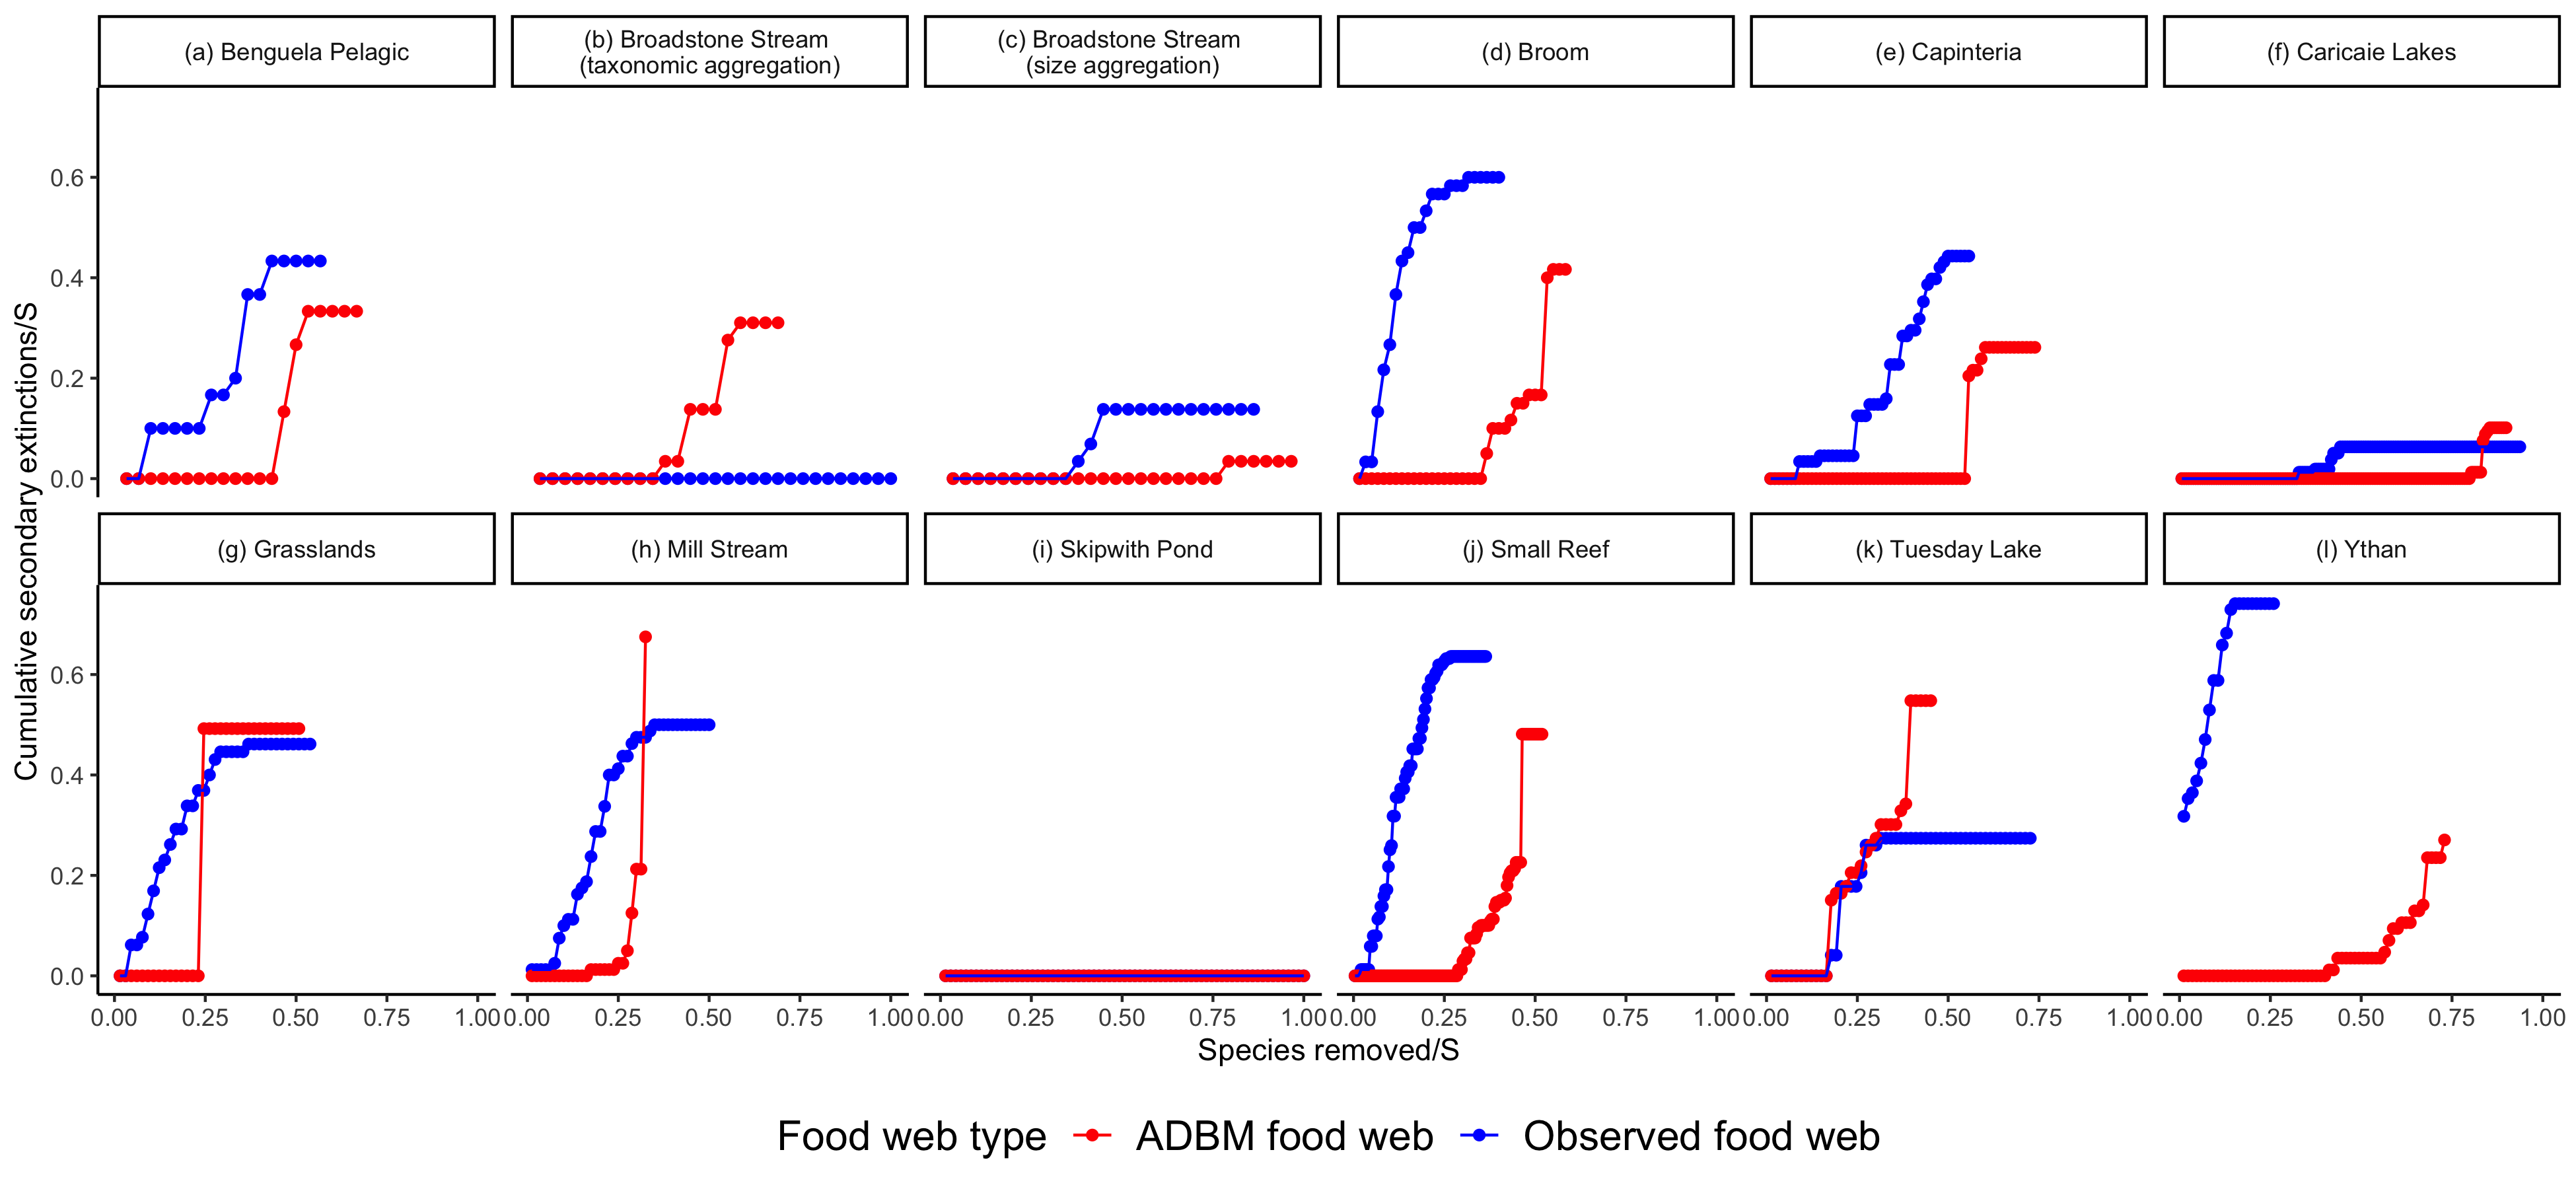
\includegraphics[width=400px]{../results/plot_mostconnected} 

}

\caption{\label{fig:fig_r1} Cumulative secondary extinctions of species resulting from the primary **removals of the most connected species** for 12 food webs. S denotes the number of species in a food web. The cumulative secondary extinctions of species and the number of species removed have been normalised by the number of species.}\label{fig:unnamed-chunk-2}
\end{figure}

Except Broadstone Stream (taxonomic aggregation), Broadstone Stream
(size aggregation) and Tuesday Lake food webs (Fig. \ref{fig:fig_r2} (b,
c and k)), the \textbf{mean cumulative secondary extinction curves}
\textbf{OP: must be explained somewhere how/why this is a mean} for all
the other food webs predicted by the ADBM were always lower than that of
the observed food webs in the random extinction scenario. The shape of
the cumulative secondary extinctions curves varied across the food webs.

\begin{figure}

{\centering 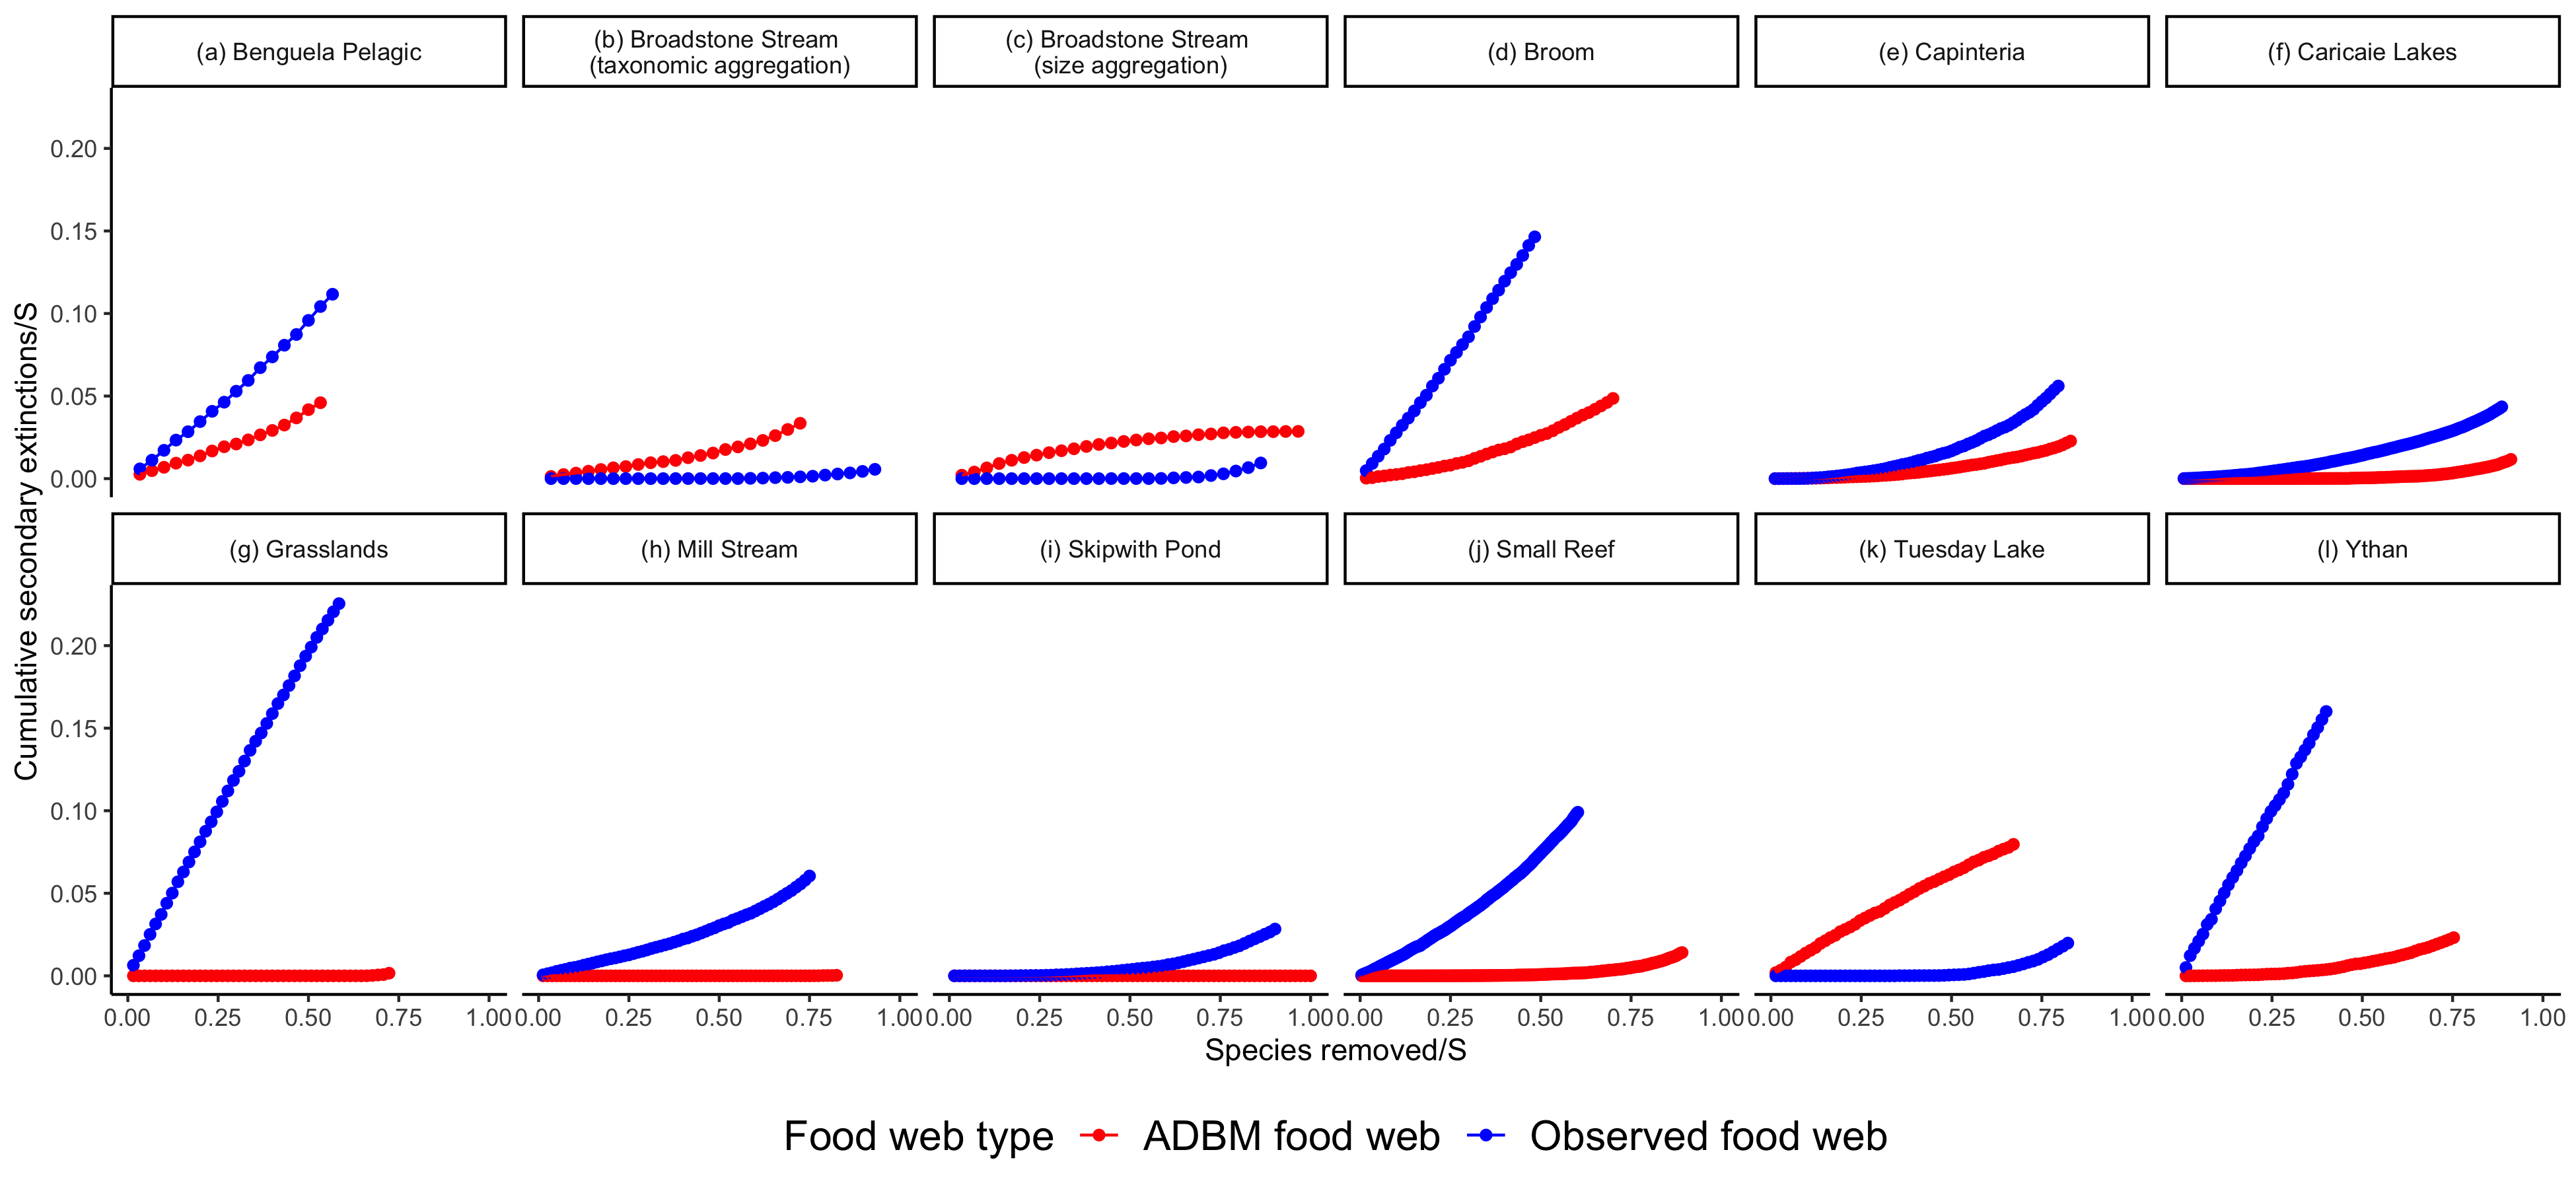
\includegraphics[width=400px]{../results/plot_random} 

}

\caption{\label{fig:fig_r2} Mean cumulative secondary extinctions of species resulting from the primary **removals of random species** for 12 food webs. S denotes the number of species in a food web. The cumulative secondary extinctions of species and the number of species removed have been normalised by the number of species.}\label{fig:unnamed-chunk-3}
\end{figure}

Compared to the most connected and random extinction scenarios, the
cumulative extinction curves in the least connected extinction scenario
had very low values and were flat for most of the food webs (Fig.
\ref{fig:fig_r3}) compared to the most connected extinction and random
extinction scenarios. In most of the food webs, there was a lot of
overlap between the extinction curves of the ADBM predicted food webs
and the observed food webs.

\begin{figure}

{\centering 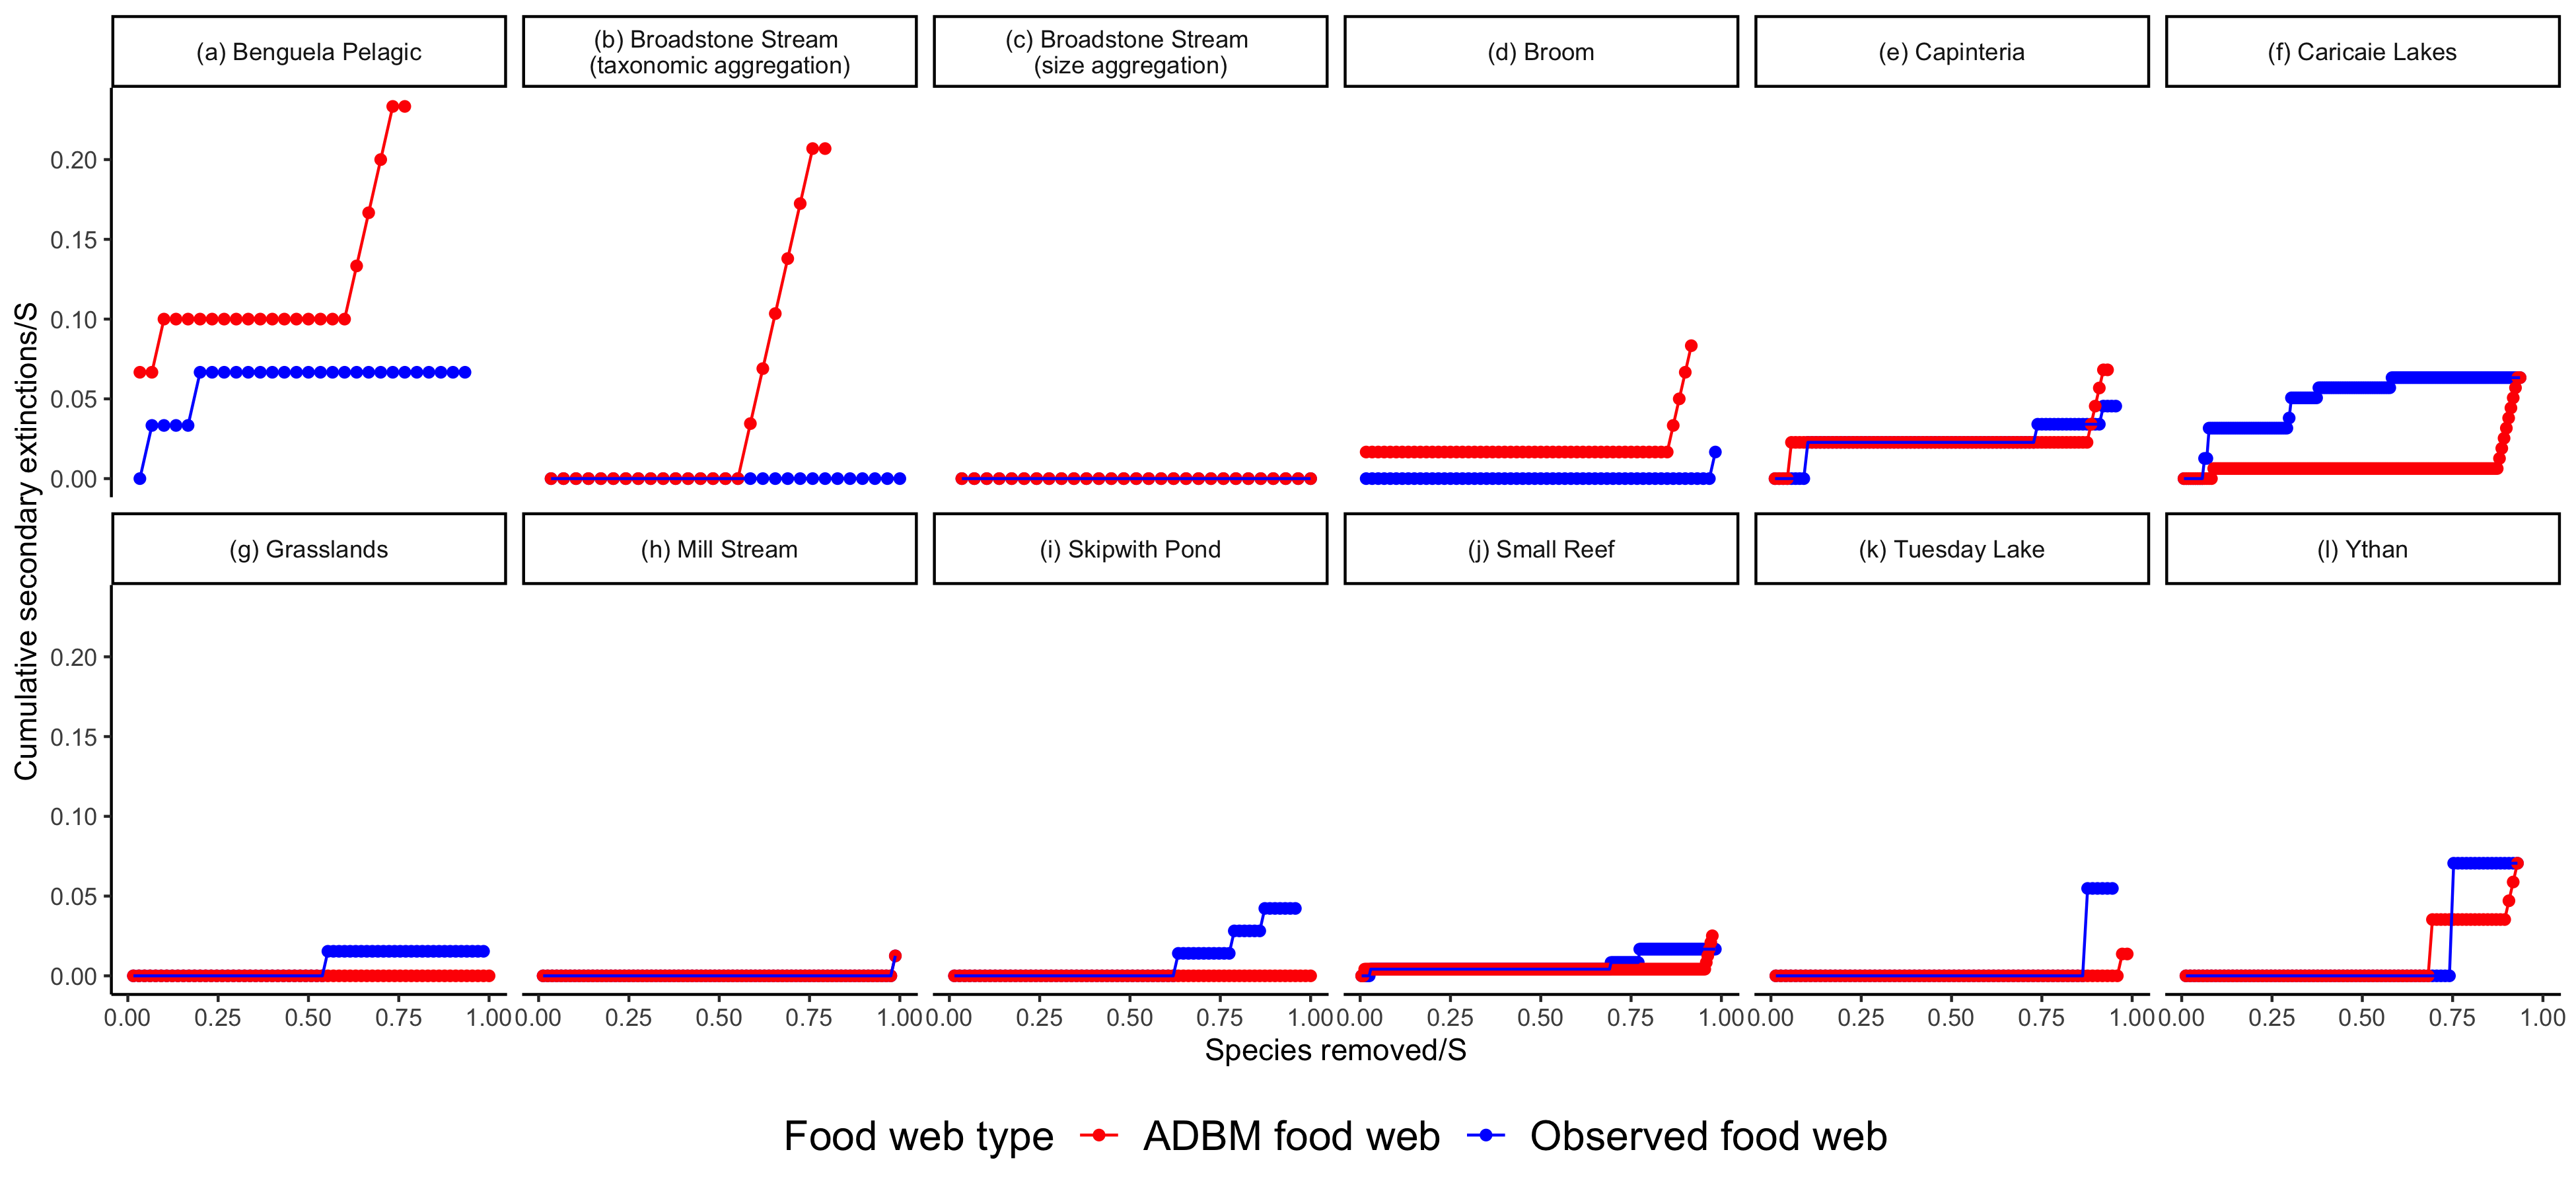
\includegraphics[width=400px]{../results/plot_leastconnected} 

}

\caption{\label{fig:fig_r3} Cumulative secondary extinctions of species resulting from the primary **removals of the least connected species** for 12 food webs. S denotes the number of species in a food web. The cumulative secondary extinctions of species and the number of species removed have been normalised by the number of species.}\label{fig:unnamed-chunk-4}
\end{figure}

\textbf{OP: write text describing the effect sizes, e.g.~how big is the
difference between observed and ADBM webs.}

\hypertarget{show-and-describe-the-following}{%
\subsection{Show and describe the
following:}\label{show-and-describe-the-following}}

I suggest to focus on the relationship between (difference in robustness
between observed and predicted connectance) and (difference in
robustness between the observed and predicted food web). \textbf{OP: I
miss text describing this relationship.} \textbf{OP: Allow the panels in
the figure to have different y-axis scales.}

\textbf{OP: This paragraph should go in the previous section}. The ADBM
predicted food webs were more robust than the observed food web with
some exceptions (Fig. \ref{fig:fig_r4}). The food webs were more robust
to least connected and random extinction scenarios than the primary
deletion of the most connected species. The difference in the robustness
values between the ADBM predicted food webs and observed food webs was
higher in the most connected extinction scenario as compared to the
least connected extinction and random extinction scenarios.

\begin{figure}

{\centering 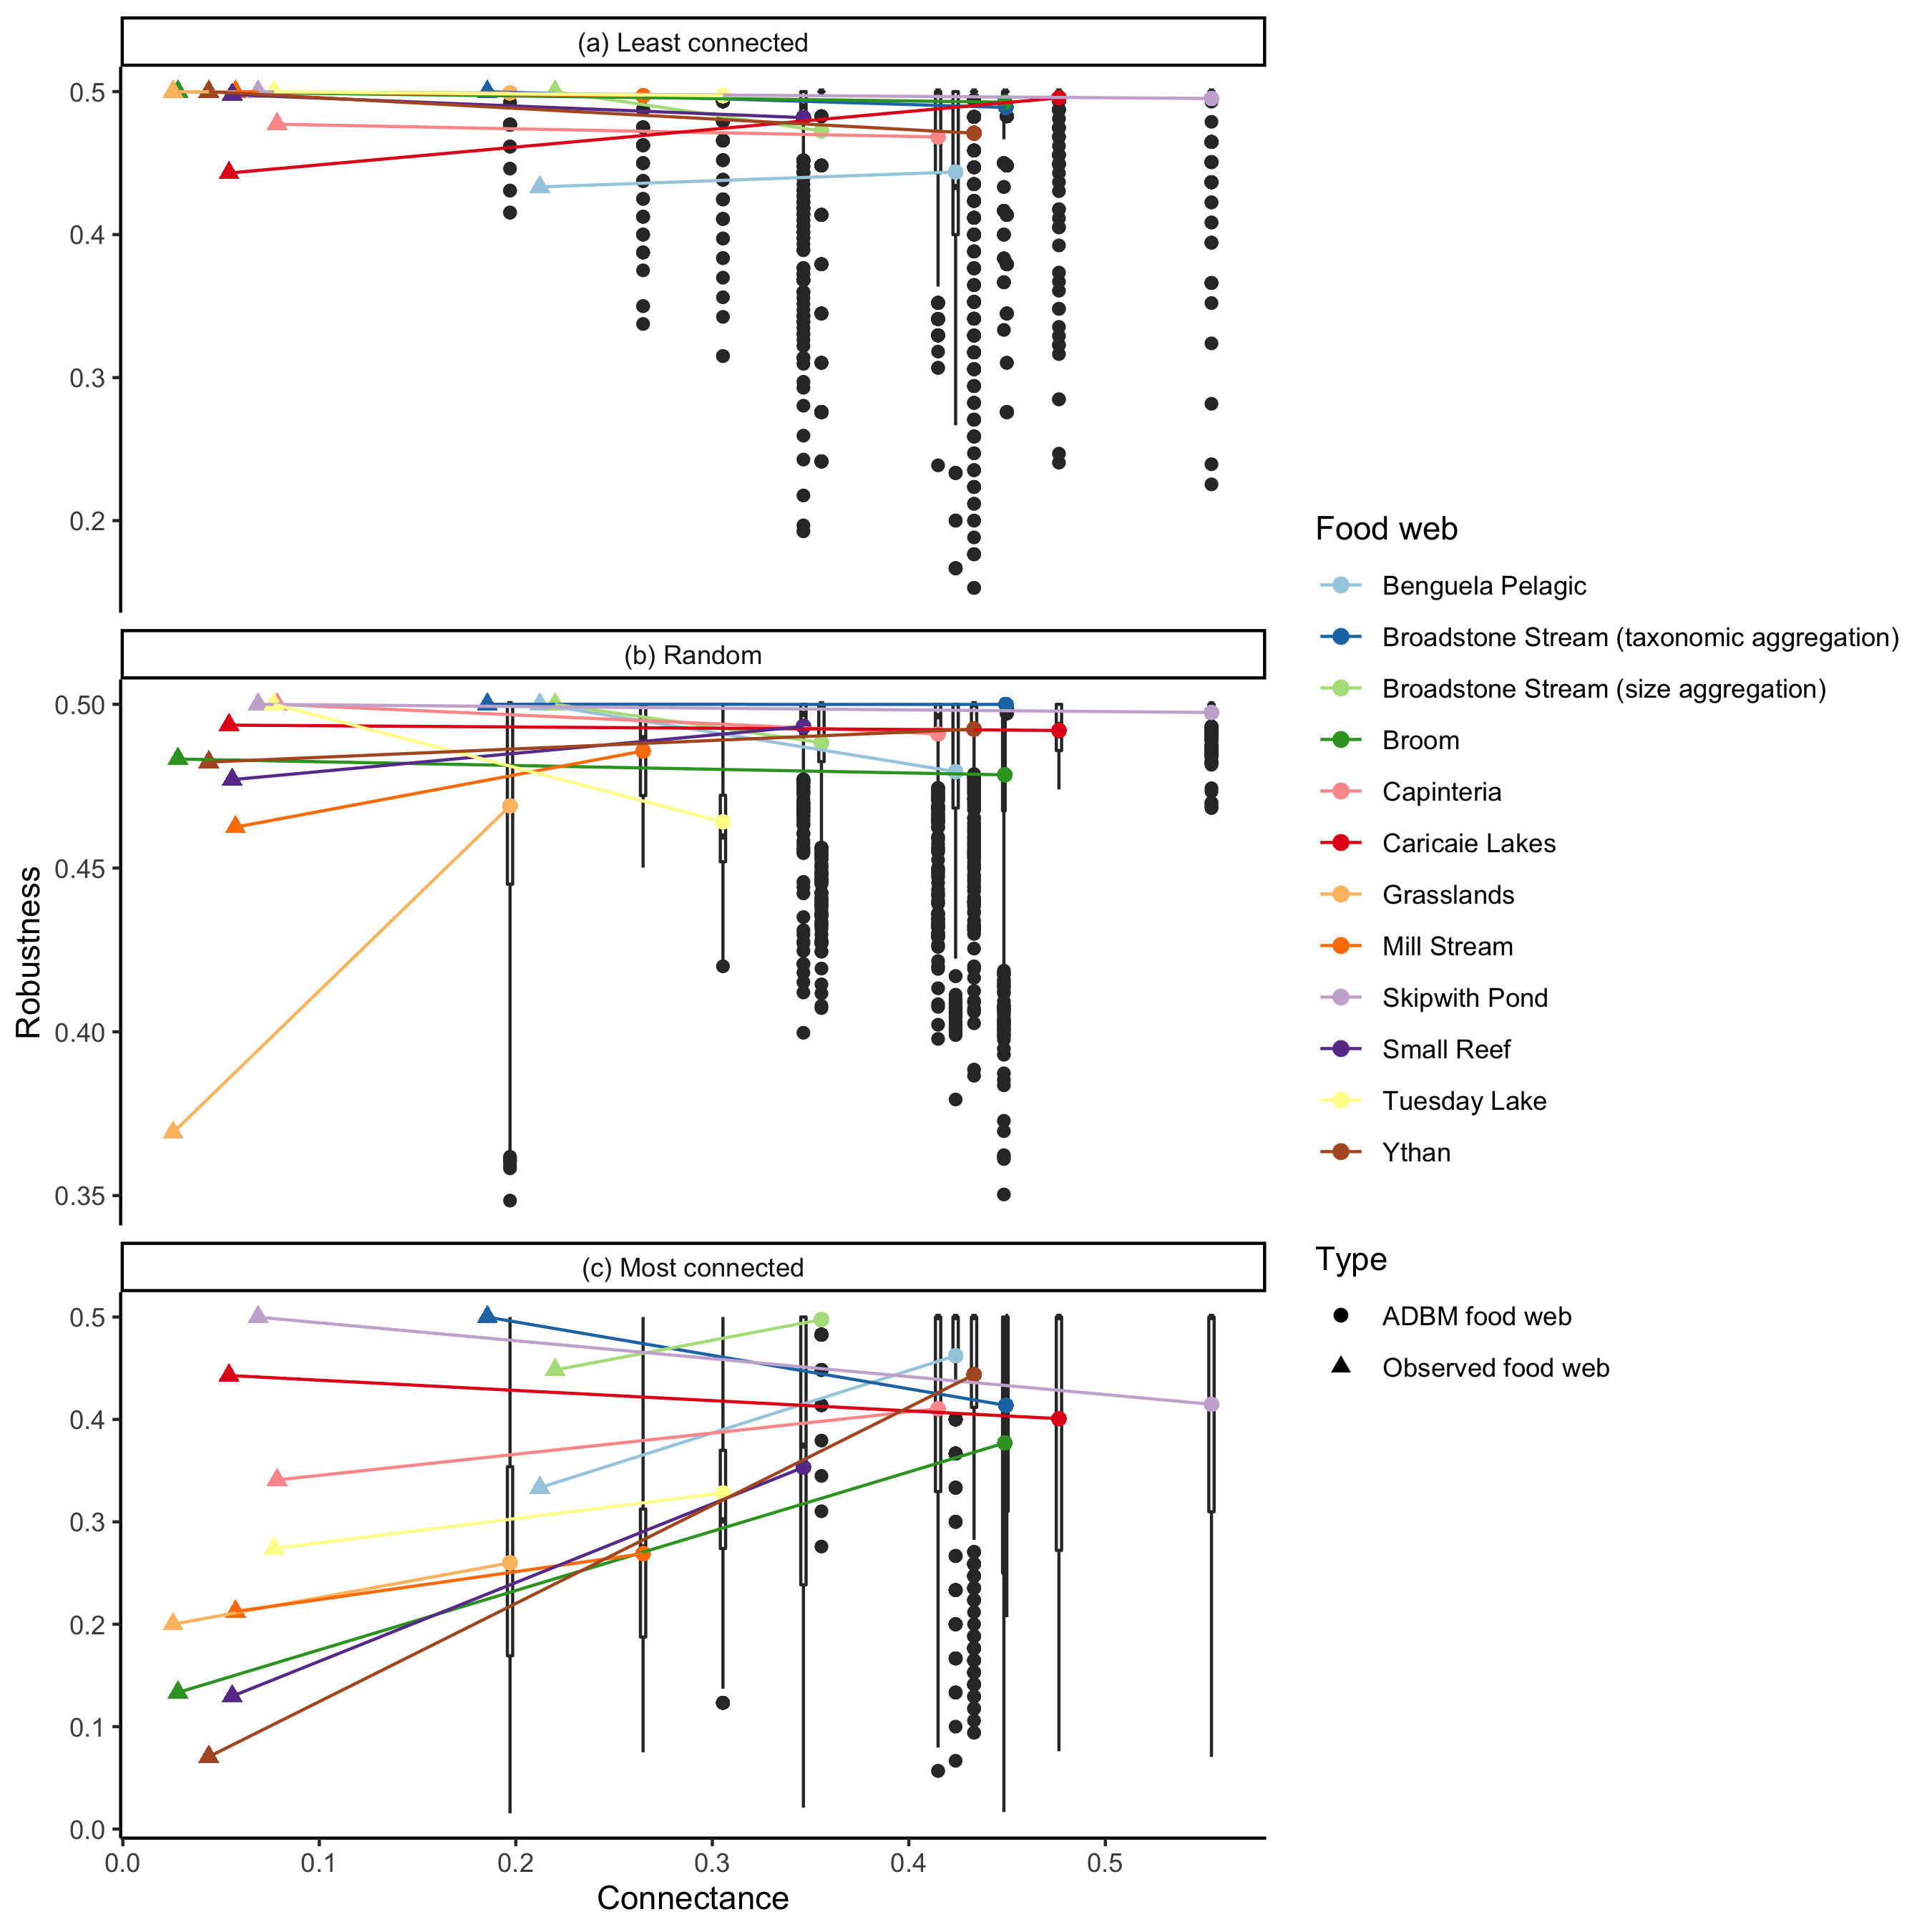
\includegraphics[width=400px]{../results/plot_robustness_all_uncertainty} 

}

\caption{\label{fig:fig_r4} Robustness plots for 12 food webs across different ecosystems. Here, $R_{50}$ is the proportion of species that have to be removed to achieve a total loss of at least 50\% of total species (primary removals and secondary extinctions).}\label{fig:unnamed-chunk-5}
\end{figure}

AG: I will also update the robustness plot for random extinction (Fig. 4
(b)) once the simulation is completed. The one shown here is only for
few simulations and as a placeholder. It takes more time to compute.

\hypertarget{discussion}{%
\section{Discussion}\label{discussion}}

The primary removal of species revealed that the ADBM predicted food
webs are more robust than the observed food webs, and the shape of the
robustness extinction curves varies between food webs.

The food webs are least robust to primary extinction of the most
connected species scenario compared to that of least connected and
random extinction scenarios. A future development would be to understand
the stability of the dynamics of the ADBM predicted food webs and
compare it with our study.

\ldots{}

\hypertarget{what-does-overestimation-of-connectance-imply-in-terms-of-stability}{%
\subsection{What does overestimation of connectance imply in terms of
stability?}\label{what-does-overestimation-of-connectance-imply-in-terms-of-stability}}

For most of the food webs, the primary removals of species resulted in a
higher secondary extinction in the ADBM predicted food webs than that of
the observed food webs (Fig. \ref{fig:fig_r1}, \ref{fig:fig_r2} and
\ref{fig:fig_r3}). This can be attributed to the higher connectance of
the ADBM predicted food webs as compared to that of the observed food
webs because a species in a food web with a high connectance has on
average more number of trophic links as compared to the food webs with
low connectance. \textbf{OP: should here cite figure 4.}

It would be intriguing to know if this difference in connectance has a
similar influence in the dynamical stability of the food webs as well.
Hence, a future prospect could be to use a dynamical model (for example:
bionergetic food web model (Brose, Williams, and Martinez 2006)) to
model the temporal dynamics of the ADBM predicted food webs. It would be
interesting to know the temporal stability of these ADBM predicted food
webs compared to the observed food webs because it has been known that
food webs with increasing connectance stability diminishes (May 1972).

\ldots{}

Include here the possibility that the increased connectance would
influence dynamical stability, and state if and why this may increase or
decrease stability.

\hypertarget{explain-that-the-adbm-can-only-predicts-contiguous-diets-op-and-the-implications-of-this}{%
\subsection{Explain that the ADBM can only predicts contiguous diets
{[}OP{]} and the implications of
this}\label{explain-that-the-adbm-can-only-predicts-contiguous-diets-op-and-the-implications-of-this}}

Using only body size as a trait, the ADBM can only predict diets that
are contiguous with respect to the size of the prey. I.e. it cannot
predict that a predator will consume prey of size 1 and 3, and not
consume prey of size 2. Also, it is important to note that the observed
diets were not contiguous when prey are ordered by their size, and this
is due to some ecological differences in how predator group choose their
prey (Caron et al. 2022). So, the parameterisation process lead to a
greater number of predicted links than observed.

This higher connectance in the ADBM predicted food webs has lead to a
higher robustness of the ADBM predicted food webs. An important question
to ask here is how reliable are these results. We suspect that both the
model and the observed data are wrong to some extent. We expect that
some of the links that do in reality occur are not present in the
observed datasets, which is quite possible because of low sampling
effort or rare prey-predator interactions even when there is intensive
sampling. This would mean that the false positives may actually be a
correctly predicted link.

We suspect that the model is also predicting links which actually do not
occur. This is because the current ADBM model only takes body size
trait, and therefore only predicts contiguous diet. That would mean any
interaction that is not possible because of some other traits not
correlated with the body size would still be predicted by the model. For
example, a species might have a defensive trait that could result in the
predator species not predating on that species at all.

AG: (Caution) Some of the texts might be very similar to or same as in
C1 MS. With multiple iterations of the current ms, the current text
would be altered. Also, the current ms would be checked using a
plagiarism software before submission.

\ldots{}

\hypertarget{compare-the-results-from-our-study-with-results-from-other-food-web-models-jennifer-a.-dunne-and-williams-2009}{%
\subsection{Compare the results from our study with results from other
food web models (Jennifer A. Dunne and Williams
(2009))}\label{compare-the-results-from-our-study-with-results-from-other-food-web-models-jennifer-a.-dunne-and-williams-2009}}

The findings from our study is similar to what had been documented for
other food web models (Jennifer A. Dunne and Williams 2009), in terms of
increase in the robustness when the connectance of the food web is
increased. A future study could be to understand the robustness of other
food web models (Gravel et al. 2013) and compare it with our study. We
expect similar results.

{[}OP{]} Including if and why we expect our findings to be replicated
with those other models. Include some of Gravel and Poissot's models

\ldots{}

\hypertarget{references}{%
\section*{References}\label{references}}
\addcontentsline{toc}{section}{References}

\hypertarget{refs}{}
\begin{CSLReferences}{1}{0}
\leavevmode\vadjust pre{\hypertarget{ref-bergUsingSensitivityAnalysis2011}{}}%
Berg, Sofia, Maria Christianou, Tomas Jonsson, and Bo Ebenman. 2011.
{``Using Sensitivity Analysis to Identify Keystone Species and Keystone
Links in Size-Based Food Webs.''} \emph{Oikos} 120 (4): 510--19.
\url{https://doi.org/10.1111/j.1600-0706.2010.18864.x}.

\leavevmode\vadjust pre{\hypertarget{ref-broseAllometricScalingEnhances2006}{}}%
Brose, Ulrich, Richard J. Williams, and Neo D. Martinez. 2006.
{``Allometric Scaling Enhances Stability in Complex Food Webs.''}
\emph{Ecology Letters} 9 (11): 1228--36.
\url{https://doi.org/10.1111/j.1461-0248.2006.00978.x}.

\leavevmode\vadjust pre{\hypertarget{ref-caronAddressingEltonianShortfall}{}}%
Caron, Dominique, Luigi Maiorano, Wilfried Thuiller, and Laura J.
Pollock. 2022. {``Addressing the {Eltonian} Shortfall with Trait-Based
Interaction Models.''} \emph{Ecology Letters} n/a (n/a).
\url{https://doi.org/10.1111/ele.13966}.

\leavevmode\vadjust pre{\hypertarget{ref-dunne2004}{}}%
Dunne, Ja, Rj Williams, and Nd Martinez. 2004. {``Network Structure and
Robustness of Marine Food Webs.''} \emph{Marine Ecology Progress Series}
273: 291--302. \url{https://doi.org/10.3354/meps273291}.

\leavevmode\vadjust pre{\hypertarget{ref-dunneCascadingExtinctionsCommunity2009}{}}%
Dunne, Jennifer A., and Richard J. Williams. 2009. {``Cascading
Extinctions and Community Collapse in Model Food Webs.''}
\emph{Philosophical Transactions of the Royal Society B: Biological
Sciences} 364 (1524): 1711--23.
\url{https://doi.org/10.1098/rstb.2008.0219}.

\leavevmode\vadjust pre{\hypertarget{ref-dunneNetworkStructureBiodiversity2002}{}}%
Dunne, Jennifer A., Richard J. Williams, and Neo D. Martinez. 2002a.
{``Network Structure and Biodiversity Loss in Food Webs: Robustness
Increases with Connectance.''} \emph{Ecology Letters} 5 (4): 558--67.
\url{https://doi.org/10.1046/j.1461-0248.2002.00354.x}.

\leavevmode\vadjust pre{\hypertarget{ref-dunne2002network}{}}%
Dunne, Jennifer A, Richard J Williams, and Neo D Martinez. 2002b.
{``Network Structure and Biodiversity Loss in Food Webs: Robustness
Increases with Connectance.''} \emph{Ecology Letters} 5 (4): 558--67.

\leavevmode\vadjust pre{\hypertarget{ref-ebenmanUsingCommunityViability2005}{}}%
Ebenman, Bo, and Tomas Jonsson. 2005. {``Using Community Viability
Analysis to Identify Fragile Systems and Keystone Species.''}
\emph{Trends in Ecology \& Evolution} 20 (10): 568--75.
\url{https://doi.org/10.1016/j.tree.2005.06.011}.

\leavevmode\vadjust pre{\hypertarget{ref-ebenmanCOMMUNITYVIABILITYANALYSIS2004}{}}%
Ebenman, Bo, Richard Law, and Charlotte Borrvall. 2004. {``{COMMUNITY
VIABILITY ANALYSIS}: {THE RESPONSE OF ECOLOGICAL COMMUNITIES TO SPECIES
LOSS}.''} \emph{Ecology} 85 (9): 2591--2600.
\url{https://doi.org/10.1890/03-8018}.

\leavevmode\vadjust pre{\hypertarget{ref-gravelInferringFoodWeb2013a}{}}%
Gravel, Dominique, Timoth'ee Poisot, Camille Albouy, Laure Velez, and
David Mouillot. 2013. {``Inferring Food Web Structure from
Predator--Prey Body Size Relationships.''} \emph{Methods in Ecology and
Evolution} 4 (11): 1083--90.
\url{https://doi.org/10.1111/2041-210X.12103}.

\leavevmode\vadjust pre{\hypertarget{ref-jordanoSamplingNetworksEcological2016}{}}%
Jordano, Pedro. 2016. {``Sampling Networks of Ecological
Interactions.''} \emph{Functional Ecology} 30 (12): 1883--93.
\url{https://doi.org/10.1111/1365-2435.12763}.

\leavevmode\vadjust pre{\hypertarget{ref-macarthur1966}{}}%
MacArthur, Robert H., and Eric R. Pianka. 1966. {``On Optimal Use of a
Patchy Environment.''} \emph{The American Naturalist} 100 (916): 603--9.
\url{https://www.jstor.org/stable/2459298}.

\leavevmode\vadjust pre{\hypertarget{ref-mayWillLargeComplex1972}{}}%
May, Robert M. 1972. {``Will a {Large Complex System} Be {Stable}?''}
\emph{Nature} 238 (5364): 413. \url{https://doi.org/10.1038/238413a0}.

\leavevmode\vadjust pre{\hypertarget{ref-patonaiAggregationIncompleteFood2017}{}}%
Patonai, Katalin, and Ferenc Jord'an. 2017. {``Aggregation of Incomplete
Food Web Data May Help to Suggest Sampling Strategies.''}
\emph{Ecological Modelling} 352 (May): 77--89.
\url{https://doi.org/10.1016/j.ecolmodel.2017.02.024}.

\leavevmode\vadjust pre{\hypertarget{ref-petchey2008}{}}%
Petchey, Owen L., A. P. Beckerman, J. O. Riede, and P. H. Warren. 2008.
{``Size, Foraging, and Food Web Structure.''} \emph{Proceedings of the
National Academy of Sciences} 105 (11): 4191--96.
\url{https://doi.org/10.1073/pnas.0710672105}.

\leavevmode\vadjust pre{\hypertarget{ref-soleComplexityFragilityEcological2001}{}}%
Sol'e, Ricard V., and M. Montoya. 2001. {``Complexity and Fragility in
Ecological Networks.''} \emph{Proceedings of the Royal Society of
London. Series B: Biological Sciences} 268 (1480): 2039--45.
\url{https://doi.org/10.1098/rspb.2001.1767}.

\leavevmode\vadjust pre{\hypertarget{ref-ullah2018}{}}%
Ullah, Hadayet, Ivan Nagelkerken, Silvan U. Goldenberg, and Damien A.
Fordham. 2018. {``Climate Change Could Drive Marine Food Web Collapse
Through Altered Trophic Flows and Cyanobacterial Proliferation.''}
Edited by Michel Loreau. \emph{PLOS Biology} 16 (1): e2003446.
\url{https://doi.org/10.1371/journal.pbio.2003446}.

\leavevmode\vadjust pre{\hypertarget{ref-williamsEffectsNetworkDynamical2008}{}}%
Williams, Richard J. 2008. {``Effects of Network and Dynamical Model
Structure on Species Persistence in Large Model Food Webs.''}
\emph{Theoretical Ecology} 1 (3): 141--51.
\url{https://doi.org/10.1007/s12080-008-0013-5}.

\end{CSLReferences}

\bibliographystyle{biblatex}
\bibliography{bibliography.bib}


\end{document}
